\documentclass{article}

\usepackage{Sweave}
\begin{document}
\Sconcordance{concordance:Lab01RinSweave.tex:Lab01RinSweave.Rnw:%
1 2 1 1 0 2 1 1 6 3 0 1 12 14 0 1 3 2 0 1 1 2 0 1 1 2 0 1 1 2 0 1 1 2 0 %
1 1 2 0 1 5 2 0 1 1 2 0 1 7 6 0 1 2 2 0 1 2 2 0 1 3 2 0 1 3 2 0 1 4 12 %
0 1 4 11 0 1 2 2 0 1 1 2 0 1 12 7 0 1 2 2 0 1 1 7 0 1 3 7 0 1 2 3 0 1 5 %
7 0 1 2 7 0 1 5 2 0 1 1 2 0 1 1 2 0 1 10 7 0 1 1 7 0 1 14 2 0 1 1 2 0 1 %
2 6 0 1 10 2 2 6 0 1 3 1 1}


\begin{Schunk}
\begin{Soutput}
[1] "H:/MSc Data Science/CMM535 - Data Science Development/Week 1 - 20200128"
\end{Soutput}
\begin{Soutput}
[1] 1 2 3 4 5
\end{Soutput}
\begin{Soutput}
 [1]  1  2  3  4  5  6  7  8  9 10
\end{Soutput}
\begin{Soutput}
[1] 1 3 5 7 9
\end{Soutput}
\begin{Soutput}
[1] "e" "s"
\end{Soutput}
\begin{Soutput}
[1]  0.0  2.5  5.0  7.5 10.0
\end{Soutput}
\begin{Soutput}
[1] "numeric"
\end{Soutput}
\begin{Soutput}
[1] 5
\end{Soutput}
\begin{Soutput}
[1] "character"
\end{Soutput}
\begin{Soutput}
[1] "numeric"
\end{Soutput}
\begin{Soutput}
 [1]  TRUE  TRUE  TRUE  TRUE  TRUE FALSE FALSE FALSE FALSE FALSE
\end{Soutput}
\begin{Soutput}
[1] FALSE FALSE FALSE FALSE FALSE
\end{Soutput}
\begin{Soutput}
 [1]  2  4  6  8 10 12 14 16 18 20
\end{Soutput}
\begin{Soutput}
 [1]  10  20  30  40  50  60  70  80  90 100
\end{Soutput}
\begin{Soutput}
     [,1] [,2] [,3] [,4]
[1,]    1    5    9   13
[2,]    2    6   10   14
[3,]    3    7   11   15
[4,]    4    8   12   16
\end{Soutput}
\begin{Soutput}
[1] 5
\end{Soutput}
\begin{Soutput}
[1] 14
\end{Soutput}
\begin{Soutput}
[1] 4 4
\end{Soutput}
\begin{Soutput}
[1] 34
\end{Soutput}
\begin{Soutput}
      [,1] [,2] [,3] [,4]
 [1,]    1   11   21   31
 [2,]    2   12   22   32
 [3,]    3   13   23   33
 [4,]    4   14   24   34
 [5,]    5   15   25   35
 [6,]    6   16   26   36
 [7,]    7   17   27   37
 [8,]    8   18   28   38
 [9,]    9   19   29   39
[10,]   10   20   30   40
\end{Soutput}
\begin{Soutput}
      [,1] [,2] [,3]
 [1,]    1   11   31
 [2,]    3   13   33
 [3,]    4   14   34
 [4,]    5   15   35
 [5,]    6   16   36
 [6,]    7   17   37
 [7,]    8   18   38
 [8,]    9   19   39
 [9,]   10   20   40
\end{Soutput}
\begin{Soutput}
[1]  7  8  9 10
\end{Soutput}
\begin{Soutput}
[1]  2.5  6.5 10.5 14.5
\end{Soutput}
\begin{Soutput}
 student_id student_name    student_grades
          1          St1         Excellent
          2          St2              Good
          3          St3               Bad
          4          St4        Really Bad
          5          St5 Really Really Bad
\end{Soutput}
\begin{Soutput}
[1] "student_id"     "student_name"   "student_grades"
\end{Soutput}
\begin{Soutput}
  student_id student_name    student_grades
1          1          St1         Excellent
2          2          St2              Good
3          3          St3               Bad
4          4          St4        Really Bad
5          5          St5 Really Really Bad
\end{Soutput}
\begin{Soutput}
  student_id    student_grades
1          1         Excellent
2          2              Good
3          3               Bad
4          4        Really Bad
5          5 Really Really Bad
\end{Soutput}
\begin{Soutput}
  student_id student_name student_grades
3          3          St3            Bad
\end{Soutput}
\begin{Soutput}
  student_id student_name    student_grades      gpa
1          1          St1         Excellent 67.59336
2          2          St2              Good 63.81619
3          3          St3               Bad 56.60937
4          4          St4        Really Bad 64.18825
5          5          St5 Really Really Bad 50.32419
\end{Soutput}
\begin{Soutput}
 student_id student_name    student_grades      gpa
          1          St1         Excellent 67.59336
          2          St2              Good 63.81619
          3          St3               Bad 56.60937
          4          St4        Really Bad 64.18825
          5          St5 Really Really Bad 50.32419
\end{Soutput}
\begin{Soutput}
Average GPA is: 	 60.50627
\end{Soutput}
\begin{Soutput}
Min GPA is: 	 50.32419
\end{Soutput}
\begin{Soutput}
Max GPA is: 	 67.59336
\end{Soutput}
\begin{Soutput}
 student_id student_name student_grades      gpa
          1          St1           Good 67.59336
          2          St2           Good 63.81619
          3          St3           Good 56.60937
          4          St4           Good 64.18825
          5          St5           Good 50.32419
\end{Soutput}
\begin{Soutput}
 student_id student_name    student_grades      gpa
          1          St1         Excellent 67.59336
          2          St2              Good 63.81619
          3          St3               Bad 56.60937
          4          St4        Really Bad 64.18825
          5          St5 Really Really Bad 50.32419
\end{Soutput}
\begin{Soutput}
[1] 42.83701
\end{Soutput}
\begin{Soutput}
[1] 38.5478
\end{Soutput}
\begin{Soutput}
 [1] 44.67955 62.81181 73.19503 27.46710 12.75139 16.51490 20.12667 78.84472
 [9] 59.56288 32.41605
\end{Soutput}
\begin{Soutput}
 [1] 44.68 62.81 73.20 27.47 12.75 16.51 20.13 78.84 59.56 32.42
\end{Soutput}
\end{Schunk}

\begin{Schunk}
\begin{Sinput}
> plot(myNumbers,squaredX,type='b',xlab = 'mynumbers', ylab = 'x*x', frame=FALSE,col='blue')
> 
\end{Sinput}
\end{Schunk}
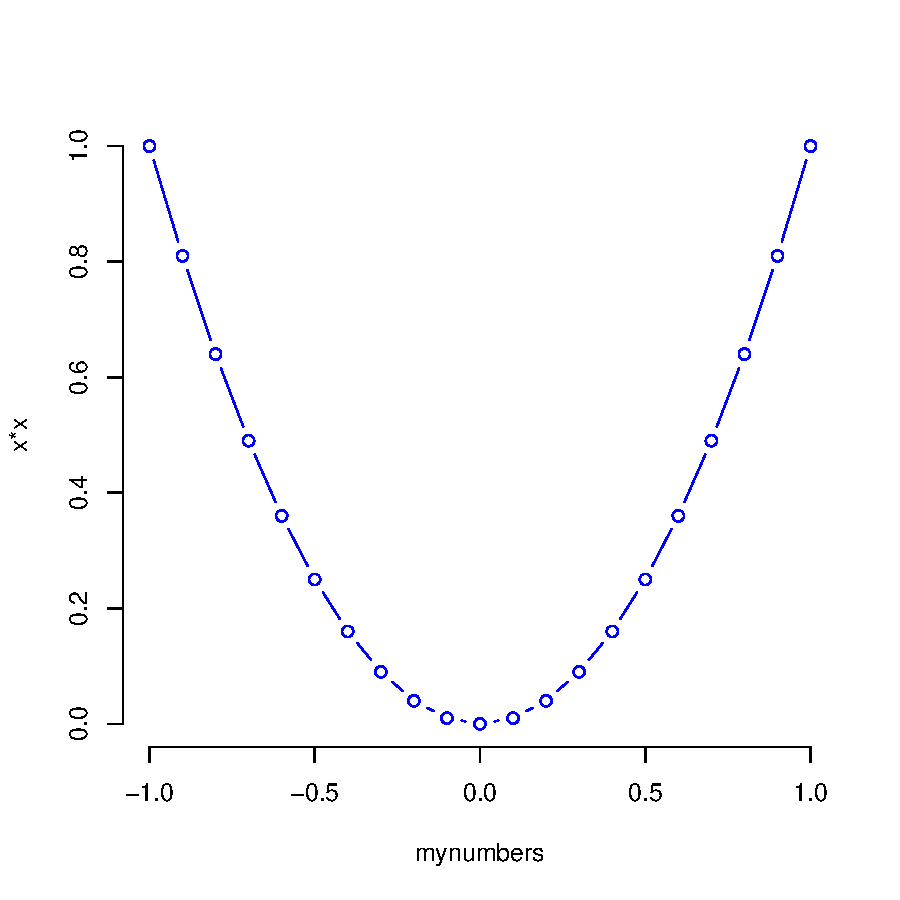
\includegraphics{Lab01RinSweave-002}

\end{document}
